% SignalConditioningCircuitry.tex
% TestingApparatus.tex
\subsection{Signal Conditioning Circuitry} % \chapter{Methodology}>\section{Prototype}
\label{subsec:SignalConditioningCircuitry}

\paragraph{Photodiodes} produce a certain amount of current when light hits the depletion region. Therefore, a larger depletion region is desirable, to capture more light and in turn produce more current. For this purpose the photodiode in our circuit is reverse-biased as can be seen in Figure \ref{fig:AltiumDis} \cite[p.155]{RefWorks:keiser2021fiber}. 

%       ~~~   TIA SUB SUB SECTION   ~~~
%
\subsubsection{\acf{TIA}}
A reverse-biased photodiode allows a current to flow from the cathode to anode which is connected to ground. This current is converted to a Voltage using a \ac{TIA} with the following relationship:
\begin{equation} \label{eq:TIAoutput} % Voltage output TIA
  \begin{split}
  V_{\text{out}} = - I_{\text{ph}} \cdot R_f
  \end{split}
\end{equation}
\addequation{Transimpedance Amplifier Output Voltage}
\begin{equation} \label{eq:Photocurrent} % Current photodiode formula
  \begin{split}
  I_{\text{ph}} = P \cdot R_{\lambda}
  \end{split}
\end{equation}
\addequation{Photocurrent as Function of Optical Power}

Where $P$ is Light Power (W) and $R_{\lambda}$ is Responsivity (A/W).

\begin{equation} \label{eq:TIAoutputWithValues}
  \begin{split}
  V_{\text{out}} = -(P \cdot 0.5 \text{ A/W}) \cdot 1 \text{ M}\Omega
  \end{split}
\end{equation}
\addequation{TIA Output with Photodiode Response}

The \ac{TIA} circuit makes use of an \ac{OpAmp} as seen in Figure \ref{fig:AltiumDis} that provides very high imput impedance (1G$\Omega$) and allows the amplification of the signal without disturbing the photodiode current, therefore not affecting the readings. The inverting input is used in this configuration, which converts the negative current flowing from the cathode to the anode of the photodiode, into a positive voltage.

% Altium Diagram
%
\begin{figure}[htbp] %h-ere t-op b-ottom p-page (separte) -good to allow all htbp to give the compiler more options
    \centering
    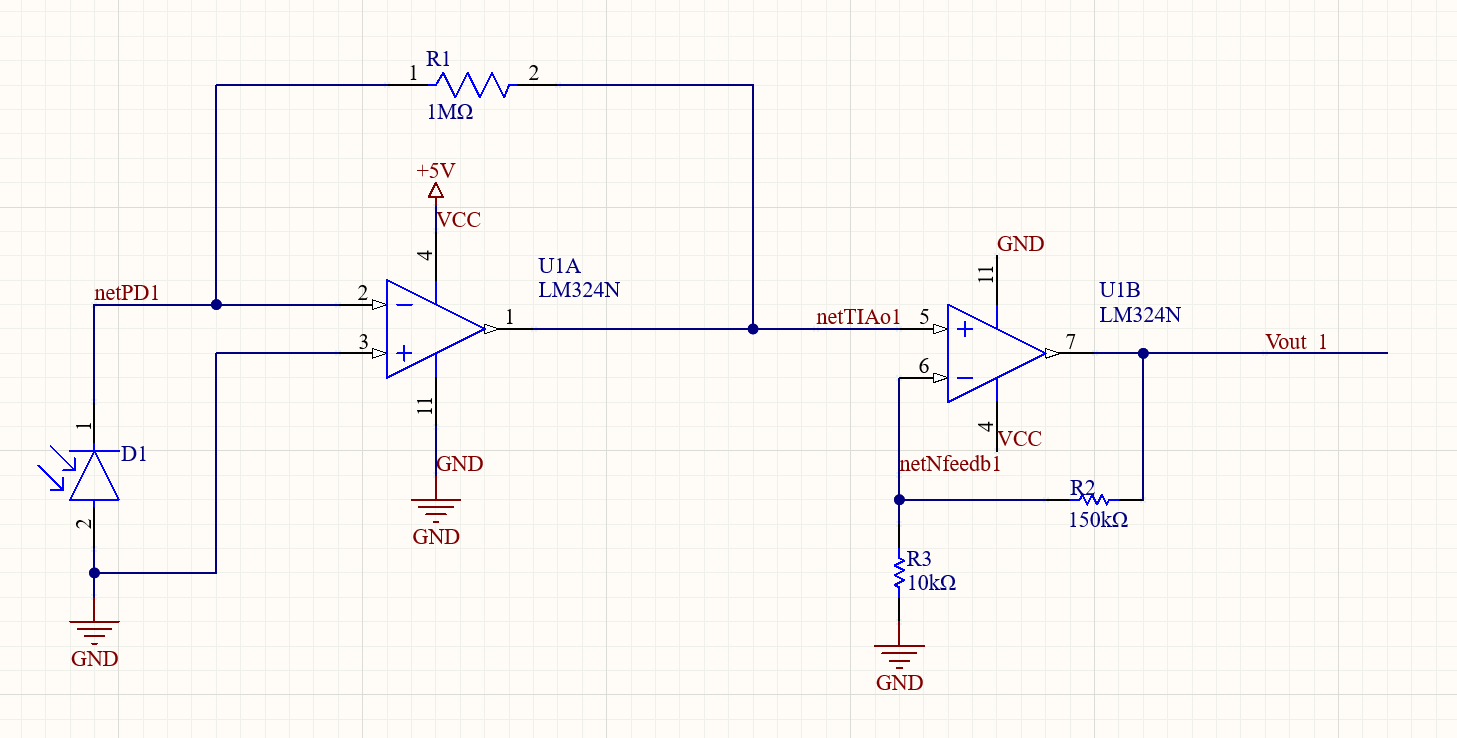
\includegraphics[width=0.8\textwidth]{chapters/methodology/prototype/AltiumSingleCircuit.png}
    \caption{TIA and Post Amplification Circuit in Altium Designer}
    \label{fig:AltiumDis}
  \end{figure}
%
%       ~~~       SECONDARY AMPLIFICATION   ~~~
%
\subsubsection{Secondary Amplification}
\label{secondAmp}
Testing showed that even using a 1M$\Omega$ resistor, the output voltage was too low (around 310mV) at our \ac{RED} testbench' \acp{LED} maximum brightness, as explained in Section \ref{explainPostAmp}. To raise the maximum Voltage to the desired maxium of the ADC of 5V, a higher feedback resistor could be used, however this would introduced noise and would require more complicated TIA with feedback capacitors. Due to the LM324-N having 4 \acp{OpAmp}, the decision was taken to implement a Secondary Amplification circuit. The non-inverting \ac{OpAmp} configuration was chosen to maintain the voltage positive, which also means there is no need for a dual power supply and keeps the Voltage positive for the Arduino ADC.
A simple calculation was made to figure out the required Gain of the circuit:
\begin{equation} \label{gainCalc}
  A = \frac{\text{required Voltage}}{\text{measured}} = \frac{5\text{ V}}{0.31\text{ V}} = 16.1
  \end{equation}
\addequation{Secondary Amplification Gain Calculation}

Knowing the gain required, the feedback resistor was calculated by choosing a 10k$\Omega R_1$ and rearranging the gain equation:

\begin{equation} \label{Feedback Resistor Calculation}
  \begin{split}
  A &= 1 + \frac{R_f}{R_1} \\
  16 &= 1 + \frac{R_f}{10\text{ k}\Omega} \\
  16 - 1 &= \frac{R_f}{10\text{ k}\Omega} \\
  15 &= \frac{R_f}{10\text{ k}\Omega} \\
  R_f &= 15 \times 10\text{ k}\Omega \\
  R_f &= 150\text{ k}\Omega
  \end{split}
\end{equation}
\addequation{Amplifier Feedback Resistor Calculation}

This provides a gain $A= 16$ which is very close to the Gain required in Equation \ref{gainCalc}. Once the design was tested on a BreadBoard, it was transfered to a stripboard as pictured in Figure \ref{fig:StripboardPhoto}.


%
% templates for figures, code, 
%

% %%% display code nicely
% \begin{lstlisting}[style=cstyle, caption=System Architecture Code Example, label=lst:SystemArchitecture7]
% # Your code here
% \end{lstlisting}

% \begin{figure}[htbp] %h-ere t-op b-ottom p-page (separte) -good to allow all htbp to give the compiler more options
%     \centering
%     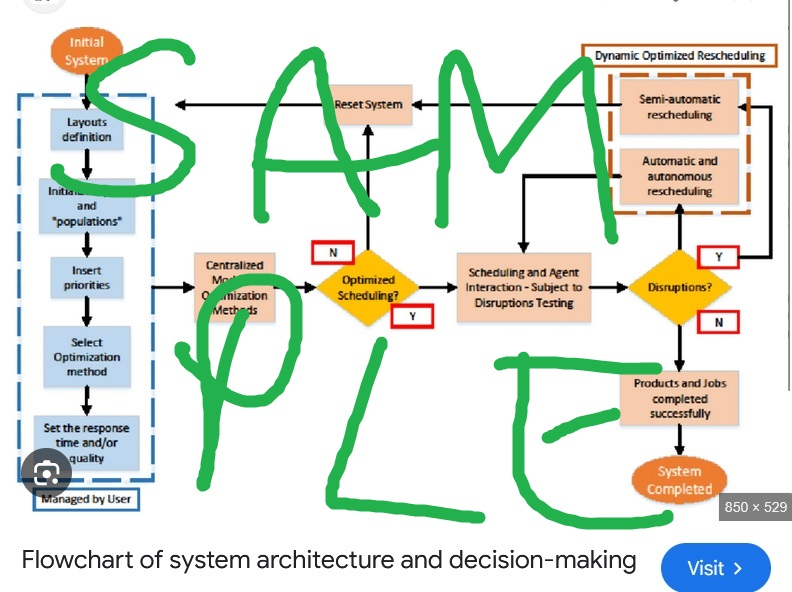
\includegraphics[width=0.6\textwidth]{figures/methodology/system_architecture.jpg}
%     \caption{System Architecture Diagram}
%     \label{fig:system-architecture2}
% \end{figure}

% % Include a flowchart in LATEX format
% \begin{figure}[H]
%     \centering
%     \scalebox{0.8}{ % Scale to 80% of original size
%         % try generating flowcharts as svg in Claude 
% and edit with inkscape instead of this.
% but claude did generate this one so might 
% be useful too but you can't easily make
% small repairs in inkscape


% CNN Transfer Learning Flowchart - Compact Multi-Column Layout
% \begin{figure}[htbp]

\centering
\resizebox{\textwidth}{!}{ % Scale to fit width while maintaining aspect ratio
\begin{tikzpicture}[node distance=0.8cm and 1.5cm, auto]
    % Define a smaller block style
    \tikzset{
      block/.style = {rectangle, draw, fill=blue!20, 
                      text width=7em, text centered, rounded corners, minimum height=1.8em, font=\small},
    }
    
    % Brazilian model training - Column 1
    \node [block] (brazildata) {Download Brazilian coins dataset};
    \node [block, below=of brazildata] (extract) {Extract dataset};
    \node [block, below=of extract] (setup) {Setup directories};
    \node [block, below=of setup] (define) {Define train/val dirs};
    \node [block, below=of define] (create) {Create CNN architecture};
    \node [block, below=of create] (compile) {Compile the CNN};
    \node [block, below=of compile] (train) {Train model};
    \node [block, below=of train] (trained) {Model trained (5 classes)};
    
    % Transfer learning - Column 2 (Middle)
    \node [block, right=2.5cm of brazildata] (freeze) {Freeze all layers};
    \node [block, below=of freeze] (replace) {Replace final layers};
    \node [block, below=of replace] (add) {Add regularization and dropout};
    \node [block, below=of add] (output) {New output layer (8 classes)};
    \node [block, below=of output] (finaltrain) {Train and fine-tune};
    \node [block, below=of finaltrain] (inference) {Perform inference on new coins};
    
    % UK data preparation - Column 3 (Right)
    \node [block, right=2.5cm of freeze] (ukdata) {Download UK coins dataset};
    \node [block, below=of ukdata] (ukextract) {Extract UK dataset};
    \node [block, below=of ukextract] (uksetup) {Setup UK directories};
    \node [block, below=of uksetup] (ukgen) {Create data generators (80/20 split)};
    
    % Connect all nodes with arrows
    \path [line] (brazildata) -- (extract);
    \path [line] (extract) -- (setup);
    \path [line] (setup) -- (define);
    \path [line] (define) -- (create);
    \path [line] (create) -- (compile);
    \path [line] (compile) -- (train);
    \path [line] (train) -- (trained);
    
    \path [line] (ukdata) -- (ukextract);
    \path [line] (ukextract) -- (uksetup);
    \path [line] (uksetup) -- (ukgen);
    
    % Connect the columns
    \path [line] (trained) -- node[midway, above] {Transfer} (freeze);
    \path [line] (ukgen) |- (finaltrain);
    
    % Connect middle column
    \path [line] (freeze) -- (replace);
    \path [line] (replace) -- (add);
    \path [line] (add) -- (output);
    \path [line] (output) -- (finaltrain);
    \path [line] (finaltrain) -- (inference);
    
    % Group boxes to show different stages with smaller padding
    \begin{pgfonlayer}{background}
        \node[group={[yshift=0.3cm]above:Brazilian Model Training}, fit={(brazildata) (extract) (setup) (define) (create) (compile) (train) (trained)}, inner sep=0.2cm] {};
        \node[group={[yshift=0.3cm]above:UK Data Preparation}, fit={(ukdata) (ukextract) (uksetup) (ukgen)}, inner sep=0.2cm] {};
        \node[group={[yshift=0.3cm]above:Transfer Learning}, fit={(freeze) (replace) (add) (output) (finaltrain) (inference)}, inner sep=0.2cm] {};
    \end{pgfonlayer}
\end{tikzpicture}
}
% \caption{CNN Transfer Learning Flowchart: Brazilian to UK Coins}
% \label{fig:cnn-flowchart}
% \end{figure}
%     }
%     \caption{System Design Overview Flowchart}
%     \label{fig:decriptiveLabel11} % descriptive to call in text with \ref{fig:decriptiveLabel}
% \end{figure}